\documentclass{article}
\usepackage{work}\usepackage{xcolor}
\usepackage{listings}
\usepackage{graphicx}
\usepackage{tikz}
\usetikzlibrary{automata, positioning}  
\usepackage{amsmath}
\def\title{Trees and Orders of Growth}
\lstset{ 
numbers = left,
  stepnumber=1,
  firstnumber = 1,
  numberfirstline = true,
  showstringspaces=false,
  language = Python 
  }
  
\begin{document}
\maketitle
\section{Introduction}
In this worksheet, we will be discussing Orders of Growth, Trees, and Objects. 
\section{Trees}
To start off, we will think about current ways that we can store data. Well all we have right now are lists, and while that's great sometimes we want to sort our data structure in one that is more organized.This is the motivation behind having a Tree data structure. 
\subsection{Tree Structure}
We will define the tree to be one that has a root and a set of children. But the question is, how do we make this? Well using our list data structure and some abstraction, we can set up a nifty tree. 
\begin{lstlisting}[language = Python]
def tree(label, branches[]):
    return [label]+branches
def label(tree):
    return tree[0]
def branches(tree):
    return tree[1:]
\end{lstlisting}
Now this may seem a bit strange, a bunch of brackets are flying around with random tree parts as the variables, so let's break it down a bit further. We will define the tree to be some arbitrary value, a number, character, ice cream bar etc. We will then define a list of branches that will serve as that particular root's children. \\*
\bigskip
Both of these items will be placed inside of a list, with the first item referring to the label and the second item referring to the branches. \\*
\bigskip
To get an idea of how exactly a tree works, let's walk through an example.
\begin{lstlisting}[language = Python]
tree(1, [2,[3], [4]],[5,[6]])
\end{lstlisting}
The above example would look like the following:
\begin{lstlisting}[language = Python]
[1, [2,[3], [4]],[5,[6]]]
\end{lstlisting}

It may be a bit confusing to see how we get from this list to a tree so let's walk through it step by step. We will start by looking at the first element of the list [1, [2,[3], [4]],[5,[6]]]. We see that 1 is our first element, so we make that the root and now have the following tree: \\*
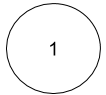
\includegraphics[scale=.34]{../images/treeex1.png}  \\*
Now that we have analyzed the 0th index of this list, let's move onto the children, [2,[3], [4]],[5,[6]]. We can see that there are 2 lists that contain all the other lists, [2,[3], [4]] and [5,[6]]. We progress by looking at the former. 2 is the first element of this list, so that means 2 will be the root of this tree. \\*
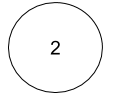
\includegraphics[scale=.34]{../images/treeex2.png}  \\*
Now we will look at the next sublist, which is just composed of [[3],[4]]. Both of these will be a tree with the root of themselves and no children, so they can be represented as follows \\*
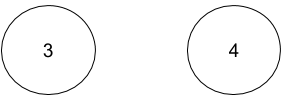
\includegraphics[scale=.34]{../images/treeex3.png}  \\*
We have no other subtrees to visualize so let's go back up. Both 3 and 4 are children of  2, so we will "connect" them to 2.\\*
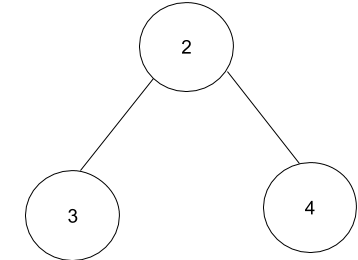
\includegraphics[scale=.34]{../images/treeex4.png}  \\*
We can do a similar process for [5,[6]] and get 2 subtrees that look as follows  \\*
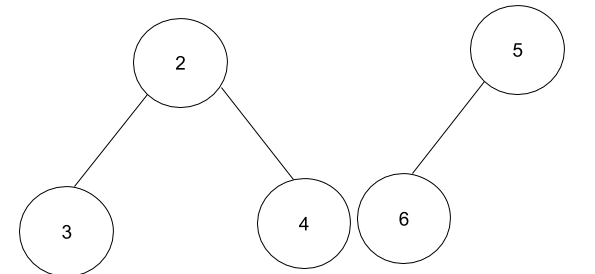
\includegraphics[scale=.34]{../images/treeex5.png} \\*
We will connect them to our initial root, 1, and then we have finished constructing our tree! \\*
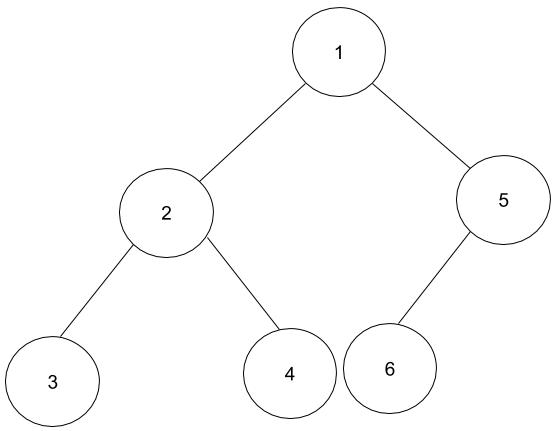
\includegraphics[scale=.34]{../images/treeexample.png}  \\*
The process of constructing trees can be a bit tedious; however, if one breaks it down systematically, it is relatively straightforward. One very important thing to remember is that a subtree of a tree is a tree itself. That is, a child of a tree is always a tree and will have a root and children, even if the children are null! 
\subsection{Utilizing Trees}
We noted that our process of constructing a tree seems to be recursive in nature. As a result, we can expect that our traversal of these structures will follow a similar process. Using our knowledge of for loops and recursion, we can come up with a skeleton that works when we want to traverse all vertices in our tree. 
\begin{lstlisting}[language = Python]
...
return [func_name(child) for child in tree.branches]
\end{lstlisting}
Basically what the above for loop does is return a new list that has the return values for all the nodes is a tree. This process tends to be used when we are constructing a new tree from our current values and simply want to do something to them (or if we want to loop over our tree for whatever reason).
\\*
\bigskip
For most tree problems, it is important to see if we are trying to make a new tree or modify the same tree. If we are trying to modify the same tree you would tend to want to use a normal for loop and modify values like that. If you want to construct a new tree then you can use a list comprehension. But regardless of the situation, we usually want to go through all the branches, which means somehow looping over them.
\section{Growth}
When writing programs, it is vital that we keep track of how fast our program runs. Working with slow, inefficient code can make your life very hard- to avoid that, we will start by learning how to analyze code. \\* \bigskip
First, we need to go over some basic rules for find the runtime of a function. 
\begin{itemize}
\item \textbf{Ignore Lower Order Terms:} When we are looking at asymptotics, we care about the highest term. This is because, as a function approaches infinity, it will be dominated by the highest order term. The proof of this can be done using some basic limit calculus so it will not be included in this document.
\item \textbf{Ignore Constants: } Given two functions of the same order, we know that they will grow at the same rate. The constant will never affect how a function grows. 
\end{itemize}
Now we will discuss the major asymptotic functions that we will discuss in the scope of this course. 
\begin{itemize}
\item $\Theta(1)$ constant time
\item $\Theta(log(n))$ logarithmic time
\item $\Theta(n)$ linear time
\item $\Theta(nlog(n))$ linearithmic time
\item $\Theta(n^{k})$ polynomial, where k is any constant number
\item $\Theta(k^{n})$ exponential, where k is any constant number.
\end{itemize}
We will briefly walk through how we can find the order of growth of some function. 
\begin{lstlisting}[language = Python]
def func(n):
	while(n > 0):
	     n-=1
	     print('hello')
	return 1
\end{lstlisting}
During each iteration of the loop we do a constant amount of work, since subtracting and print are both constant time operations. However, this loop runs a total of n times, which means that we run a total of $\Theta(n*1)$ times so $\Theta(n)$ times.
\newpage
\section{Questions}
\subsection{FunRuntime}
Find the runtime of the following function in terms of n.
\begin{lstlisting}[language = Python]
def fun(n):
	count = n
	while(n > 0):
	     n-=1
	return fun(count-1)
\end{lstlisting}
\bigskip
\bigskip
\bigskip
\bigskip
\bigskip
\bigskip
\bigskip
\bigskip
\subsection{Liebonacci}
The basic fibonacci code is written as follows: 
\begin{lstlisting}[language = Python]
def fib(n):
	if(n <= 2):
	     return n
	return fib(n-1)+fib(n-2)
\end{lstlisting}
However, this code is very inefficient, it runs in $\Theta(2^{n})$ time. Write a better version of fibonacci that can run in linear time. You can use any exterior variables,arguments, or methods. 
This solution uses a technique called caching. Instead of throwing away the data you've used, you store it. This way, you have a significantly less number of calls to your function.
\bigskip
\bigskip
\bigskip
\bigskip
\bigskip
\bigskip
\bigskip
\bigskip
\bigskip
\bigskip
\bigskip
\bigskip
\bigskip
\bigskip
\bigskip
\bigskip
\subsection{FibTree}
As you can tell, we are obsessed with the Fibonacci sequence. As a result, we will attempt to create a Fibonacci tree as follows: \\*
\bigskip
The argument passed in will be n, which refers to the nth fibonacci number. We want each number below a node to be the two numbers that compose it. For example, for n = 4 we have \\*
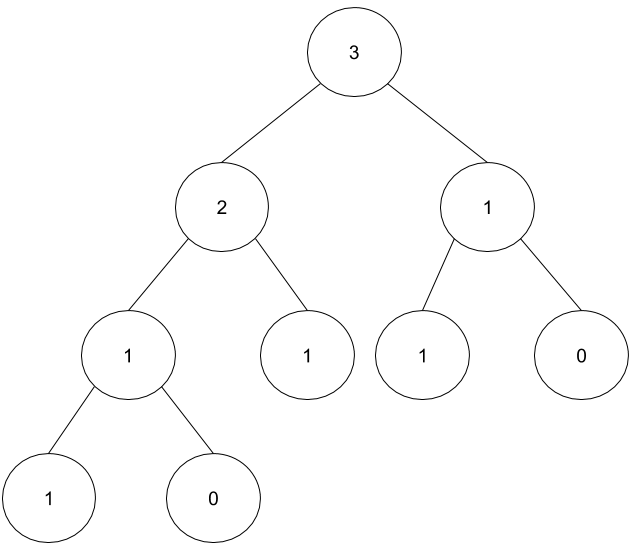
\includegraphics[scale=.35]{../images/fibtree} \\*
The top number is the 4th fibonacci number. It's children and the 3rd and 2nd fibonacci number, and this process continues until we reach the 0th and 1st fibonacci numbers. 
\bigskip
\bigskip
\bigskip
\bigskip
\bigskip
\bigskip
\bigskip
\bigskip
\bigskip
\bigskip
\bigskip
\bigskip
\bigskip
\bigskip
\bigskip
\bigskip
\bigskip
\bigskip
\bigskip
\bigskip
\bigskip
\bigskip
\bigskip
\bigskip
 \subsection{Tree Diggers}
 Write a function that, given a tree, will find the height (the root is at the 0th height) of it and see if there is a node in the tree that is equal to it. You are limited to making one pass through the tree, meaning you cannot visit the vertices more than once.
\bigskip
\bigskip
\bigskip
\bigskip
\bigskip
\bigskip
\bigskip
\bigskip
\bigskip
\bigskip
\bigskip
\bigskip
\bigskip
\bigskip
\bigskip
\bigskip
\newpage
\section{Solutions}
\subsection{FunRuntime}
Find the runtime of the following function in terms of n.
\begin{lstlisting}[language = Python]
def fun(n):
	count = n
	while(n > 0):
	     n-=1
	return fun(count-1)
\end{lstlisting}
\begin{solution}
This runs in $\Theta(n^{2})$. We do a total of n recursive calls, and we are upper bounded by n work per call. You may be wondering how we're getting $n^{2}$ as it intuitively just seems like less. Well we do n work in the first call, n -1 in the second... and 1 in the last. So if we rewrite this we can get n+n-1+...1 = 1+2+...n-1+n = $n^{2}$ by identity.
\end{solution}
\subsection{Liebonacci}
The basic fibonacci code is written as follows: 
\begin{lstlisting}[language = Python]
def fib(n):
	if(n <= 2):
	     return n
	return fib(n-1)+fib(n-2)
\end{lstlisting}
However, this code is very inefficient, it runs in $\Theta(2^{n})$ time. Write a better version of fibonacci that can run in linear time. You can use any exterior variables,arguments, or methods. 
\begin{solution}
\begin{lstlisting}[language = Python]
cache = {}
def fib(n):
    if(n <2):
         return n
    if(n-1 not in cache):
    	 cache[n-1] = fib(n-1)
    if(n-2 not in cache):
        cache[n-2] = fib(n-2)
    return cache[n-1]+ cache[n-2]
\end{lstlisting}
This solution uses a technique called caching. Instead of throwing away the data you've used, you store it. This way, you have a significantly less number of calls to your function.
\end{solution}
\subsection{FibTree}
As you can tell, we are obsessed with the Fibonacci sequence. As a result, we will attempt to create a Fibonacci tree as follows: \\*
\bigskip
The argument passed in will be n, which refers to the nth fibonacci number. We want each number below a node to be the two numbers that compose it. For example, for n = 4 we have \\*
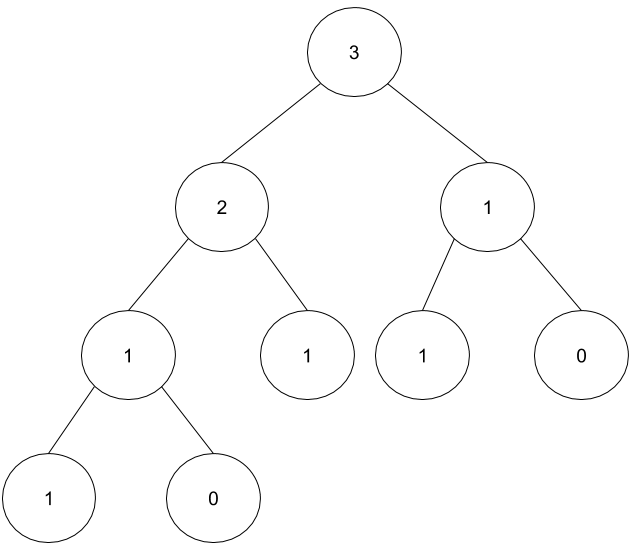
\includegraphics[scale=.35]{../images/fibtree} \\*
The top number is the 4th fibonacci number. It's children and the 3rd and 2nd fibonacci number, and this process continues until we reach the 0th and 1st fibonacci numbers. 
\begin{solution}
\begin{lstlisting}[language = Python]
def fibTree(n):
    if( n < 2):
        return Tree(n)
    else:
        left = fibTree(n-1)
        right = fibTree(n - 2)
        return Tree(left.entry + right.entry, [left, right])
\end{lstlisting}
We do the same thing as normal fibonacci, except we recursive create a tree while doing so. The major difficulty was probably wrapping your head around the tree abstraction. 
\end{solution}
 \subsection{Tree Diggers}
 Write a function that, given a tree, will find the height (the root is at the 0th height) of it and see if there is a node in the tree that is equal to it. You are limited to making one pass through the tree, meaning you cannot visit the vertices more than once.
 \begin{solution}
 \begin{lstlisting}[language = Python]
def treeDepth(t):
    i = 0
    l = []
    deepness = depth(t, 0, l)
    while(i < len(l)):
        if(l[i] == deepness):
            return True
        else:
            return False

def depth(t, count=0, l=[]):
        l += [t.entry]
        if(not t.branches):
            return count
        lst = []
        for b in t.branches:
            lst+=[depth(b,count+1,l)]
        return max(lst)
\end{lstlisting}
We utilized a helper function to find the depth of the tree. We passed in a list as an argument, and since we modified the same list throughout our tree traversal, the object in our initial class had all the modification. From here we simply go through our list and see if any values match with out tree values.
 \end{solution}
\end{document}